\documentclass[12pt,3p]{article}
\usepackage[utf8]{inputenc}
\usepackage[english]{babel}
 \usepackage[margin=0.5in]{geometry}
 \usepackage{amsmath}
 \usepackage{amssymb}
\usepackage{mathtools}
\usepackage{enumitem}
\usepackage{xcolor}		% For different colored text 
\usepackage{listings}	% For code text 
\usepackage[round,numbers]{natbib}
\usepackage[colorlinks = false]{hyperref}
\usepackage{graphicx}
\usepackage{subcaption}

\numberwithin{equation}{section}

\begin{document}

%====================================================================================
%====================================================================================
%====================================================================================
%====================================================================================
\title{Personal Notes on Paper: \\
	\large{Crack tip fields in soft elastic solids subjected to large quasi-static deformation}}
\author{Rong Long, Chung-Yuen Hui}
\date{\vspace{-5ex}}
\maketitle

\tableofcontents
\newpage

%====================================================================================
%====================================================================================
%====================================================================================
\section{Definitions}
$y_\alpha$ where $\alpha = 1, 2$ are deformed coordinates \\
$(r, \theta)$ are polar coordinates \\
$m_{\alpha}, p_{\alpha}$ are unknown exponents \\
$v_{\alpha} (\theta), q_{\alpha} (\theta)$unknown functions describing the angular variation \\ \\
$I$ ? \\
$A, B$ are material constants \\
$n$ is a material constant where $n = 1$ recovers a neo-Hookean or Mooney-Rivlin material \\
$\mu$ is the small strain shear modulus \\ \\
$a, b_0$: unknown positive amplitude \\
$U (\theta, n)$: dimensionless function \\
$H (\theta, n)$: angular function \\
$F$ is a hypergeometric function \\ 

%====================================================================================
%====================================================================================
%====================================================================================
\section{Geometry, Notations, and Basic Equations}

%====================================================================================
%====================================================================================
\subsection{Governing Equations: Kinematics and Equilibrium}
In-plane displacements because we are considering plane-strain, plane-stress, and anti-plane shear
\begin{equation}
u_{\alpha}\left(X_{1}, X_{2}\right)=x_{\alpha}\left(X_{1}, X_{2}\right)-X_{\alpha} \quad \alpha=1,2
\end{equation}
In the plane-stress formulation, ($X_1, X_2$) denote the mid-plane coordinates of a material point in the undeformed reference configuration. The undeformed crack tip is at the origin, $X_1 = X_2 = 0$\\ \\
Introduction of $y_\alpha$ definition for considering displacement of the crack tip: 
\begin{equation}
y_{\alpha}\left(X_{1}, X_{2}\right) \equiv x_{\alpha}\left(X_{1}, X_{2}\right)-x_{\alpha}\left(X_{1}=0, X_{2}=0\right)
\end{equation}
Therefore, considering we are given displacements from Paraview
\begin{align}
y_{\alpha}\left(X_{1}, X_{2}\right) &=  (u_{\alpha}\left(X_{1}, X_{2}\right) +X_{\alpha}) - (u_{\alpha}\left(0, 0 \right) +X_{\alpha} (0, 0)) \\
&= u_{\alpha}\left(X_{1}, X_{2}\right) - u_{\alpha} (0, 0) + X_{\alpha} - X_{\alpha} (0,0)
\end{align}

%====================================================================================
%====================================================================================
%====================================================================================
\section{Crack tip fields under large deformations}

%====================================================================================
%====================================================================================
\subsection{Method of asymptotic analysis}
The deformed coordinates, $y_1 \, y_2$, were assumed to be a series consisting of separable functions of the polar coordinates ($r, \theta$) in the undeformed material in the vicinity of the crack tip 
\begin{equation}
\begin{array}{l}
y_{a}(r, \theta)=r^{m_{a}} v_{a}(\theta)+r^{n_{0}} q_{a}(\theta)+\cdots \\
m_{a}<p_{a}, \quad \alpha=1,2
\end{array}
\end{equation}
where $m_\alpha, p_\alpha$ are unknown exponents and $v_\alpha (\theta). q_\alpha (\theta)$ are unknown functions describing the angular variation

%====================================================================================
%====================================================================================
\subsection{Plane strain crack in homogeneous materials}
Strain energy density 
\begin{equation}
W(I \gg 1)=A I^{n}+B I^{n-1}+o\left(l^{n-1}\right)
\end{equation}
$n$ is a material constant where $n = 1$ recovers a neo-Hookean or Mooney-Rivlin material. Remove higher order terms. 
\begin{align*}
W(I \gg 1) &=A I^{1} + B I^{1-1} + o (l^{1-1}) \\
W(I \gg 1) &=A I + B \quad \text{where} \, A = \frac{\mu}{2} \, B = - \frac{3 \mu}{2} \\
		&= \frac{\mu}{2} I - \frac{3 \mu}{2} \\
W(I \gg 1) &= \frac{\mu}{2} (I - 3)
\end{align*}

%====================================================================================
\subsubsection{Crack tip deformation field (Mode I)}
The characteristics of the deformation has a transition at n = 3/2. Note that n=1 indicates a Neo-Hookan material. 
\begin{align}\label{EqDisp}
\begin{split}
y_{1} &= \left\{\begin{array}{ll}
-b_{0} r^{2-\frac{1}{n}}[U(\theta, n)]^{2}, & 1 / 2<n<3 / 2 \\
-\frac{1}{a} r^{1+\frac{1}{2 \pi}} H(\theta, n), & n>3 / 2
\end{array}\right. \\
y_2 &= a r^{1 - \frac{1}{2n}} U (\theta, n) 
\end{split}
\end{align}
U is simply a dimensionless function that holds for any n 
\begin{align}\label{EqU}
U (\theta, n) = \sin \bigg( \frac{\theta}{2} \bigg) \sqrt{1-\frac{2 \kappa^{2} \cos ^{2}(\theta / 2)}{1+\omega(\theta, n)}} \times[\omega(\theta, n)+\kappa \cos \theta]^{\kappa / 2}, \quad 0 \leq|\theta| \leq \pi
\end{align}
where 
\begin{equation}\label{EqKappa}
\kappa = 1 - \frac{1}{n}
\end{equation}
\begin{equation}\label{EqOmega}
\omega (\theta, n) = \sqrt{1 - (\kappa \, \sin \theta)^2}
\end{equation}
H is an angular function that is only relevant for n $>$ 3/2 \textcolor{red}{Note that we have a typo where it is written that n $>$ 3/2}
\begin{equation}
H(\theta, n) = -\frac{n^{5 / 2}}{m^{2}}[\omega(\theta, n)+ \kappa \cos \theta]^{2-m} \bigg[ \frac{m}{2-m} \times F \bigg(\frac{1}{2}-\frac{1}{m}, \frac{1}{2} ; \frac{3}{2}-\frac{1}{m} ; \cos ^{2} \xi_{0} \bigg) -\kappa \sin \xi_{0} \bigg]
\end{equation}
where F is the hypergeometric function and, 
\begin{align*}
m &= 1 - \frac{1}{2n} \\
\cos \xi_{0} &= \frac{1}{n \sqrt{2}} \frac{\sqrt{1+k \sin ^{2} \theta-\omega(\theta, n) \cos \theta}}{\omega(\theta, n)+\kappa \cos \theta} 
\quad \quad 0 \leq \xi_{0} \leq \frac{\pi}{2}
\end{align*}
To make sure I have plotted correctly, check the boundaries 
\begin{align*}
H(\theta=0, n) &= -\frac{4 n^{9 / 2}}{(2 n-1)^{2}}\left[2-\frac{1}{n}\right]^{1+\frac{1}{2 m}} \frac{1}{n(2 n+1)} \\
H(\theta = \pm \pi, n) &= -\frac{4 n^{9 / 2}}{(2 n-1)^{2}} n^{-1-\frac{1}{n}}\left(\frac{2 n-1}{2 n+1}\right) \times \frac{\sqrt{\pi} \Gamma\left(\frac{2 n-3}{2(2 n-1)}\right)}{\Gamma\left(\frac{-1}{2 n-1}\right)}
\end{align*}
where the gamma function exists in MATLAB. \\
\begin{figure}[h]
    \centering
    \begin{subfigure}[b]{0.45\textwidth}
        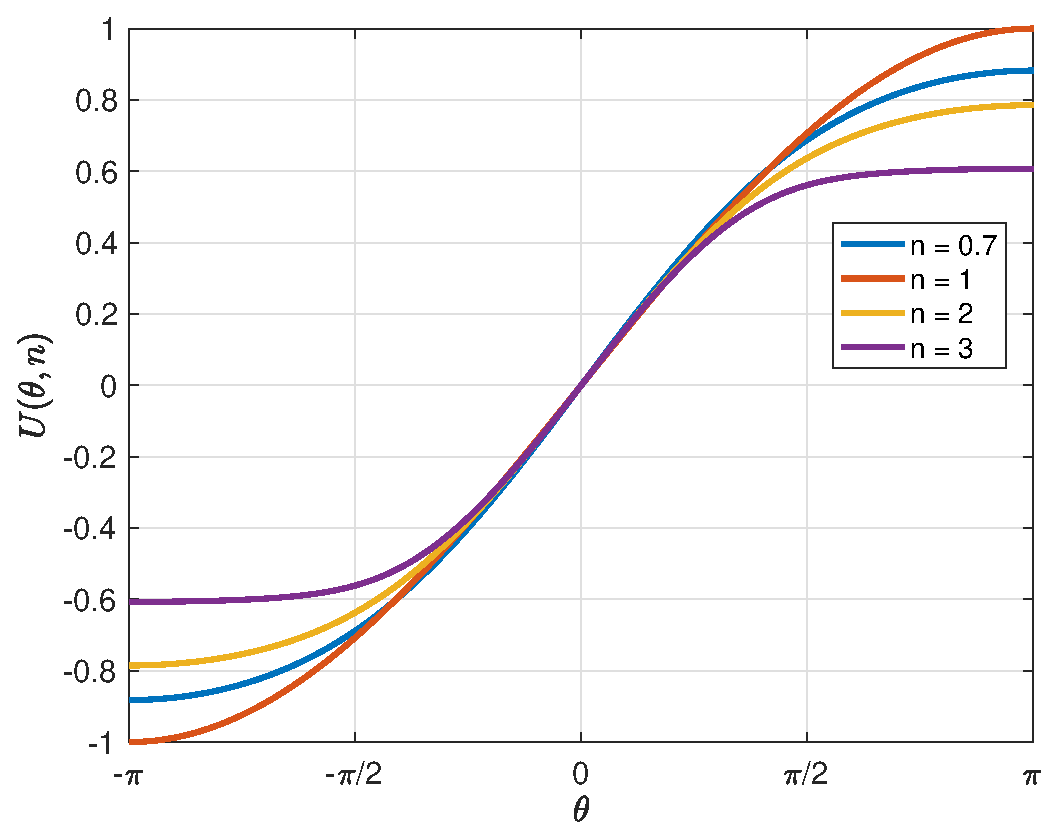
\includegraphics[width=\textwidth]{Fig3A.eps}
    \end{subfigure}
    \quad %add desired spacing between images, e. g. ~, \quad, \qquad, \hfill etc. 
    \begin{subfigure}[b]{0.45\textwidth}
        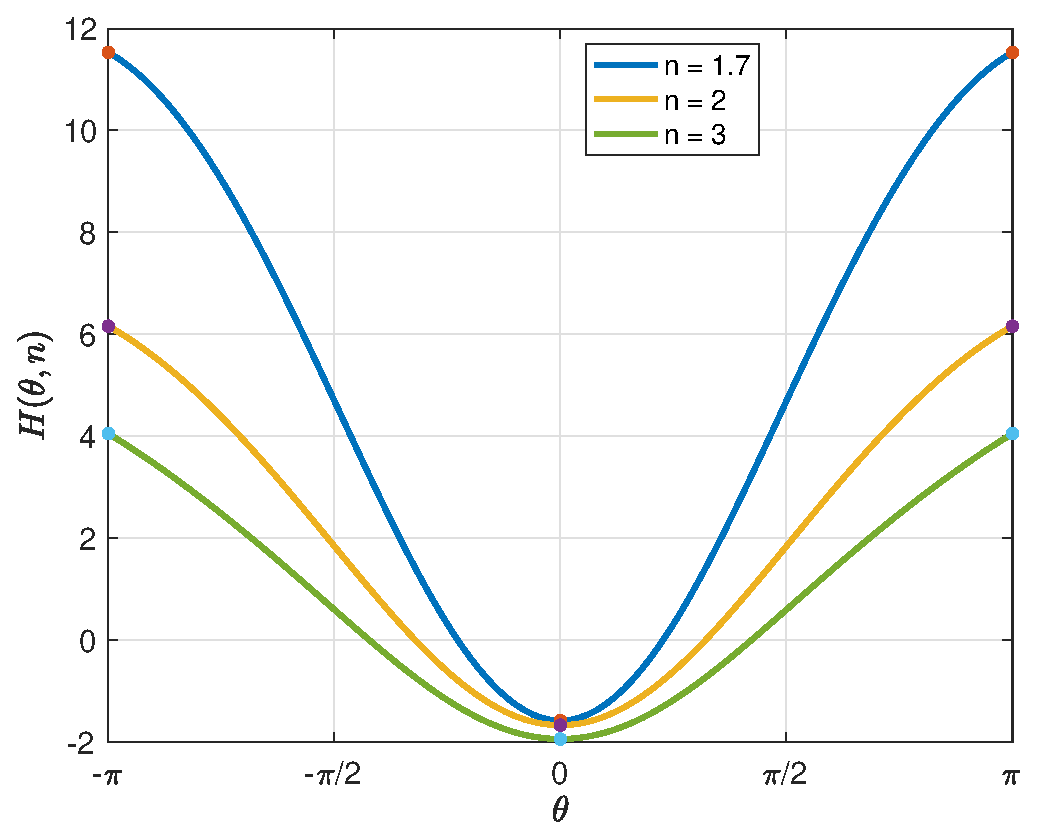
\includegraphics[width=\textwidth]{Fig3B.eps}
    \end{subfigure}
    \caption{Replication of Figure 3 without n = 10}
\end{figure}
\noindent\rule{\linewidth}{0.5pt} % Straight line across 
Note that plotting U in Fig 3A is simply a matter of choosing a n value and using Eq. \ref{EqU}, \ref{EqKappa}, and \ref{EqOmega}. Plotting H is more complicated and relies on inbuilt functions in MATLAB for hypergeometric and Gamma functions, for example 
\begin{lstlisting}
for i = 1:length(x)
   F(i) = hypergeom([1/2 - 1/m, 1/2], 3/2 - 1/m, x(i));
end
\end{lstlisting}
and to check the boundaries, we list two gamma functions as follows: 
\begin{lstlisting}
gamma1 = gamma((2*n(ii)-3)/(2*(2*n(ii)-1)));
gamma2 = gamma(-1/(2*n(ii)-1));
\end{lstlisting}
\noindent\rule{\linewidth}{0.5pt} % Straight line across 
In the interest of replicating Figure 4A, rewrite the equations for the deformed coordinates near the crack tip, where we are interested in n between 1/2 and 3/2
\begin{align}\label{EqCoord}
\begin{split}
y_1 &= -b_{0} r^{2-\frac{1}{n}}[U(\theta, n)]^{2} \\
y_2 &= a r^{1 - \frac{1}{2n}} U (\theta, n) 
\end{split}
\end{align}
Before normalizing the result, we first rearrange $y_2$
\begin{align*}
\frac{y_2}{a} = r^{1 - \frac{1}{2n}} U (\theta, n) 
\end{align*}
and substitute into $y_1$
\begin{align}
y_1 &= -b_{0} r^{2-\frac{1}{n}} [U(\theta, n)]^{2} \\
	&= -b_{0} r^{2(1 - \frac{1}{2n})} [U(\theta, n)]^{2} \\
y_1 &= -b_0 \bigg( \frac{y_2}{a} \bigg)^2
\end{align}
Therefore, we now have Eq. 40a in the paper
\begin{align}\label{Eq40a}
y_1 &= -b_0 \bigg( \frac{y_2}{a} \bigg)^2 \\
\sqrt{\frac{y_1}{-b_0}} &= \frac{y_2}{a} \\
\pm a \sqrt{\frac{y_1}{-b_0}} &= y_2 
\end{align}
Now if we normalize by $a^{2n}$, where normalized quantities are denoted by $(\hat{})$
\begin{align}
\begin{split}
\hat{y}_1 &= - \frac{b_{0}}{a^{2n}} r^{2-\frac{1}{n}}[U(\theta, n)]^{2} \quad \quad \hat{y}_2 = \frac{a}{a^{2n}} r^{1 - \frac{1}{2n}} U (\theta, n) \\
\hat{y}_1 &= - \frac{b_{0}}{a^{2n}} r^{2-\frac{1}{n}}[U(\theta, n)]^{2} \quad \quad \hat{y}_2 = a^{1-2n} r^{1 - \frac{1}{2n}} U (\theta, n) \\
\hat{y}_1 &= - \frac{x a^{2-2n}}{a^{2n}} r^{2-\frac{1}{n}}[U(\theta, n)]^{2} \\
\hat{y}_1 &= - x a^{2-4n} r^{2-\frac{1}{n}}[U(\theta, n)]^{2} 
\end{split}
\end{align}
where we can introduce some unknown x according to the figure caption: 
\begin{equation}
x = \frac{b_0}{a^{2-2n}} \rightarrow b_0 = x a^{2-2n}
\end{equation}
Finally
\begin{equation}
\hat{y}_1 = - x (\hat{y}_2)^2 = - \frac{b_0}{a^{2-2n}} (\hat{y}_2)^2 
\end{equation}

%====================================================================================
\subsubsection{Special case: n = 1 for neo-Hookean or MR solid}
First, we want to plot U for n = 1, which makes $\kappa = 0$ and $\omega = 1$
\begin{align*}
U (\theta, n) &= \sin (\frac{\theta}{2}) \sqrt{1-\frac{2 \kappa^{2} \cos ^{2}(\theta / 2)}{1+\omega(\theta, n)}} \times[\omega(\theta, n) + \kappa \cos \theta]^{\kappa / 2}, \quad 0 \leq|\theta| \leq \pi \\
		&= \sin (\frac{\theta}{2}) \sqrt{1-\frac{2 (0) \cos ^{2}(\theta / 2)}{2}} \times[ 1 + \cos \theta]^{0/2} \\ 
U (\theta, 1) &= \sin (\frac{\theta}{2}) 
\end{align*}
Therefore, considering n = 1, starting with Eq. \ref{EqCoord}, we can obtain Eq. 48 in the paper
\begin{align*}
y_1 &= -b_{0} r^{2-\frac{1}{n}} [U(\theta, n)]^{2} = -b_{0} r \bigg[\sin (\frac{\theta}{2}) \bigg]^2 \\ 
y_2 &= a r^{1 - \frac{1}{2n}} U (\theta, n) = a \sqrt{r} \sin (\frac{\theta}{2}) 
\end{align*}
In terms of the normalized quantities, we have the following: 
\begin{align}
\begin{split}
\hat{y}_1 &= - x a^{2-4n} r^{2-\frac{1}{n}}[U(\theta, n)]^{2} \quad \quad \hat{y}_2 = a^{1-2n} r^{1 - \frac{1}{2n}} U (\theta, n) \\
\hat{y}_1 &= - x a^{2-4} r^{2-1}[U(\theta, 1)]^{2} \quad \quad \hat{y}_2 = a^{1-2} r^{1 - \frac{1}{2}} U (\theta, 1) \\
\hat{y}_1 &= - b_0 a^{-2} r \bigg[\sin (\frac{\theta}{2}) \bigg]^{2} \quad \quad \hat{y}_2 = a^{-1} \sqrt{r} \sin (\frac{\theta}{2}) \\
\hat{y}_1 &= - b_0 \hat{y}_2^2
\end{split}
\end{align}
\noindent\rule{\linewidth}{0.5pt} % Straight line across 
There are several ways to plot Fig. 4, but I plotted the full U function for more generalizability. In the MATLAB code, we simply set the value of x which is a ratio of $b_0$ and $a$. 
\begin{align*}
\hat{y}_2 &= \frac{1}{a} \sqrt{r} \, U (\theta, 1) \\
\hat{y}_1 &= -x \hat{y}_2^2
\end{align*}
\textcolor{red}{Note: neglect the $\frac{\sqrt{r}}{a}$ in the actual code:}
\begin{lstlisting}
y2 = real(U);
y1 = -x(ii)*y2.^2;
\end{lstlisting}
How this is plotted in Figure 4 is by setting n = 1 for the calculation of $\kappa$ for $U$
\begin{figure}[h!]
	\centering
        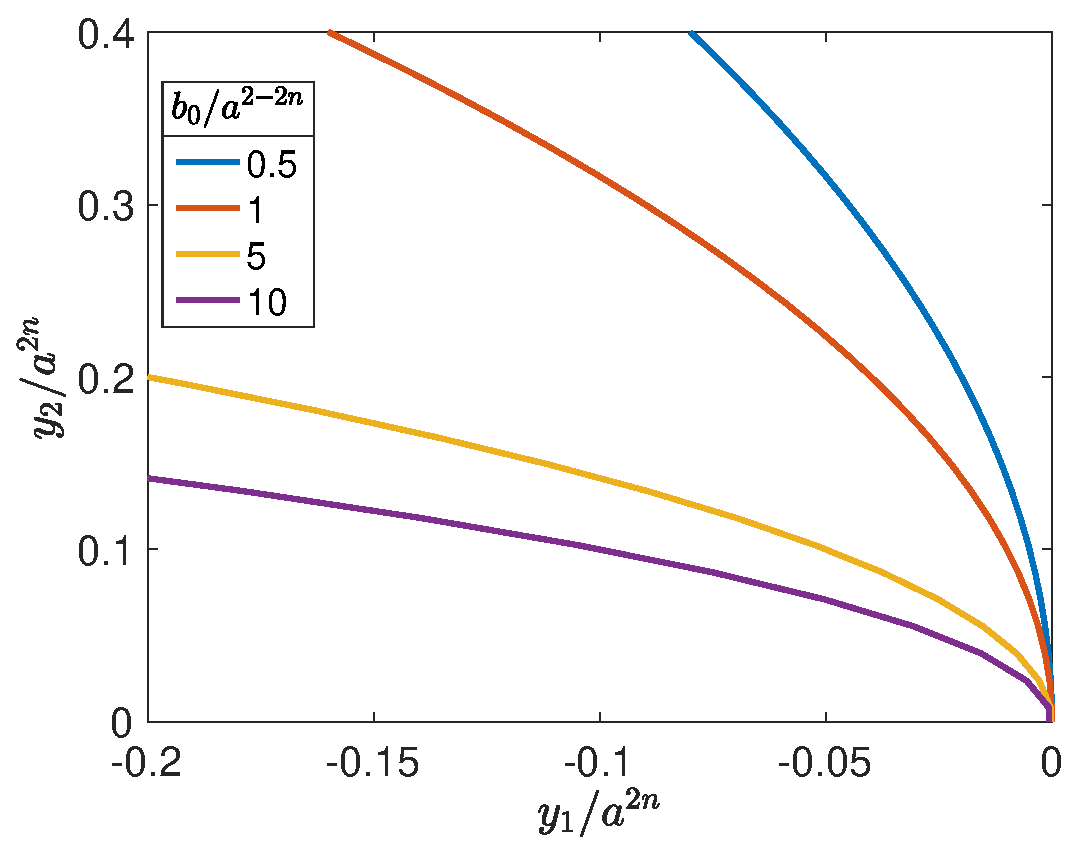
\includegraphics[width=0.5\textwidth]{Fig4A.eps}
        \caption{Crack opening profile predicted by the asymptotic solution.}
\end{figure}

%====================================================================================
%====================================================================================
\subsection{Plane stress crack in homogenous materials}

%====================================================================================
\subsubsection{Crack tip deformation field for GNH solids}
Leading order terms of mode I deformation field $y_1$ and $y_2$: 
\begin{align}
y_1 &= c r^d g (\theta, n), \, d < 1 + \frac{1}{4n} \quad \quad n < n^* \\
y_2 &= a r^{1-\frac{1}{2n}} U(\theta, n)
\end{align}
For the special case of a neo-Hookean solid with n = 1 
\begin{align}
d = 1 \quad \text{and} \quad g(\theta, n = 1) = \cos \theta
\end{align}

%====================================================================================
\subsubsection{Special case: n = 1 for neo-Hookean solid}
Therefore for a neo-Hookean solid we obtain Eq. 65 in the paper
\begin{align*}
y_1 &= c r \cos \theta \\
y_2 &= a \sqrt{r} \sin \bigg( \frac{\theta}{2} \bigg)
\end{align*}
\noindent\rule{\linewidth}{0.5pt} % Straight line across 
\textcolor{red}{Note 1: There is a distinct difference in the relation between $y_1$ and $y_2$ see Eq. 66 below} 
\begin{align*}
y_2 &= \pm a \sqrt{\frac{- y_1}{c}} \\
\bigg( \frac{y_2}{a} \bigg)^2 &= \frac{-y_1}{c} \\
c r \sin^2 \bigg( \frac{\theta}{2} \bigg) = - y_1 
\end{align*}
but $ - \cos (\theta) \neq \sin^2 (\theta/2)$ \\
\noindent\rule{\linewidth}{0.5pt} % Straight line across 
If we want to plot this similarly to Fig. 3 in the paper, we normalize by $a^{2n}$ or $a^{2}$ for n = 1 
\begin{align*}
\hat{y}_1 = \frac{c}{a^{2n}} r \cos \theta \\
\hat{y}_1 = \frac{c}{a^2} r \cos \theta \rightarrow r = \frac{\hat{y}_1 a^2}{c \cos \theta}
\end{align*}
For $\hat{y}_2$ we substitute the above identity for r \\
\begin{align*}
\hat{y}_2 &= a^{1-2n} \sqrt{r} \sin \bigg( \frac{\theta}{2} \bigg) \\
\hat{y}_2^2 &= a^{-2} r \sin^2 \bigg( \frac{\theta}{2} \bigg) \quad \text{where} \, \sin^{2} \bigg( \frac{\theta}{2}\bigg) = \frac{1}{2} (1 - \cos \theta) \\
\hat{y}_2^2 &= a^{-2} r \frac{1}{2} (1 - \cos \theta) \quad \text{substitute r} \\
\hat{y}_2^2 &= a^{-2} \frac{\hat{y}_1 a^2}{c \cos \theta} \frac{1}{2} (1 - \cos \theta) \\
\hat{y}_2^2 &=  \frac{1}{2c} \frac{(1 - \cos \theta)}{\cos \theta} \hat{y}_1
\end{align*}
Rearrange so we obtain the following properties: 
\begin{align*}
\hat{y}_1 = 2 c \hat{y}_2^2 \frac{\cos \theta}{1 - \cos \theta} \quad \hat{y}_2 = \frac{1}{a}\sqrt{r} \sin \bigg( \frac{\theta}{2}\bigg) 
\end{align*}
\textcolor{red}{Note 2: we can determine a but not c.}

%====================================================================================
%====================================================================================
%====================================================================================
\section{Energetics: J-integral and energy release rate}
The J-integral for plane stress, Mode I opening 
\begin{align*}
J &= \frac{\mu \pi}{2} \bigg( \frac{b}{n} \bigg)^{n-1} \bigg( \frac{2n - 1}{2n} \bigg)^{2n - 1} n^{1-n} a^{2n} \quad n = 1 \\
J &= \frac{\mu \pi a^{2}}{4}
\end{align*}

%====================================================================================
%====================================================================================
\subsection{Interpretation of J-integral in experiments}
For a pure shear specimen the J-integral is
\begin{align}\label{PureShearJInt}
J = 2 W (I_1, I_2) h_0 = 2 \Psi (\lambda_A) h_0
\end{align}
where the stretch in the direction of loading is: 
\begin{align*}
\lambda_A = 1 + \frac{\Delta}{h_0}
\end{align*}
For a neo-hookean solid 
\begin{align*}
\Psi = \frac{\mu}{2} (\lambda_A - \lambda_A^{-1})^2
\end{align*}
where we can substitute this into the J-integral Eq. \ref{PureShearJInt} and solve for a 
\begin{align*}
J &= 2 \Psi (\lambda_A) h_0 \\
J &= \mu (\lambda_A - \lambda_A^{-1})^2 h_0 \\
\frac{\mu \pi a^{2}}{4} &= \mu (\lambda_A - \lambda_A^{-1})^2 h_0 \\
a^{2} &= \frac{4h_0}{\pi} (\lambda_A - \lambda_A^{-1})^2 \\
a &= 2 \sqrt{\frac{h_0}{\pi}} (\lambda_A - \lambda_A^{-1})
\end{align*}
The unknown amplitude c decreases monotonically from 1.55 at $\lambda_A = 1.02$ to 1.15 at $\lambda_A = 2$. 

\end{document}